    \stepcounter{Plenarycounter} %counter increase
    % formatting table of contents entry    
    \addcontentsline{toc}{section} 
    { 
		%\arabic{Plenarycounter} 
			{Self-focusing of the flow: On the growth of karst conduits and river networks} \\ 			
    \normalfont\small Piotr Szymczak }
    % end -- formatting table of contents entry 
    
    { \centering{ \textsc{ \textbf{ \large{Self-focusing of the flow: On the growth of karst conduits and river networks}} } } \\    
    } 
      { \centering{ \textbf{ 
				Piotr Szymczak} \\ 
    %\blfootnote{Corresponding author: Bayode Owolabi, e-mail: \href{mailto:sgbowola@liverpool.ac.uk}{sgbowola@liverpool.ac.uk} }
  Faculty of Physics, University of Warsaw, Poland\\ 
	} } 
	\vspace{1cm} 
	\begin{wrapfigure}{r}{4cm}
		\vspace{-20pt}
		\begin{center}
			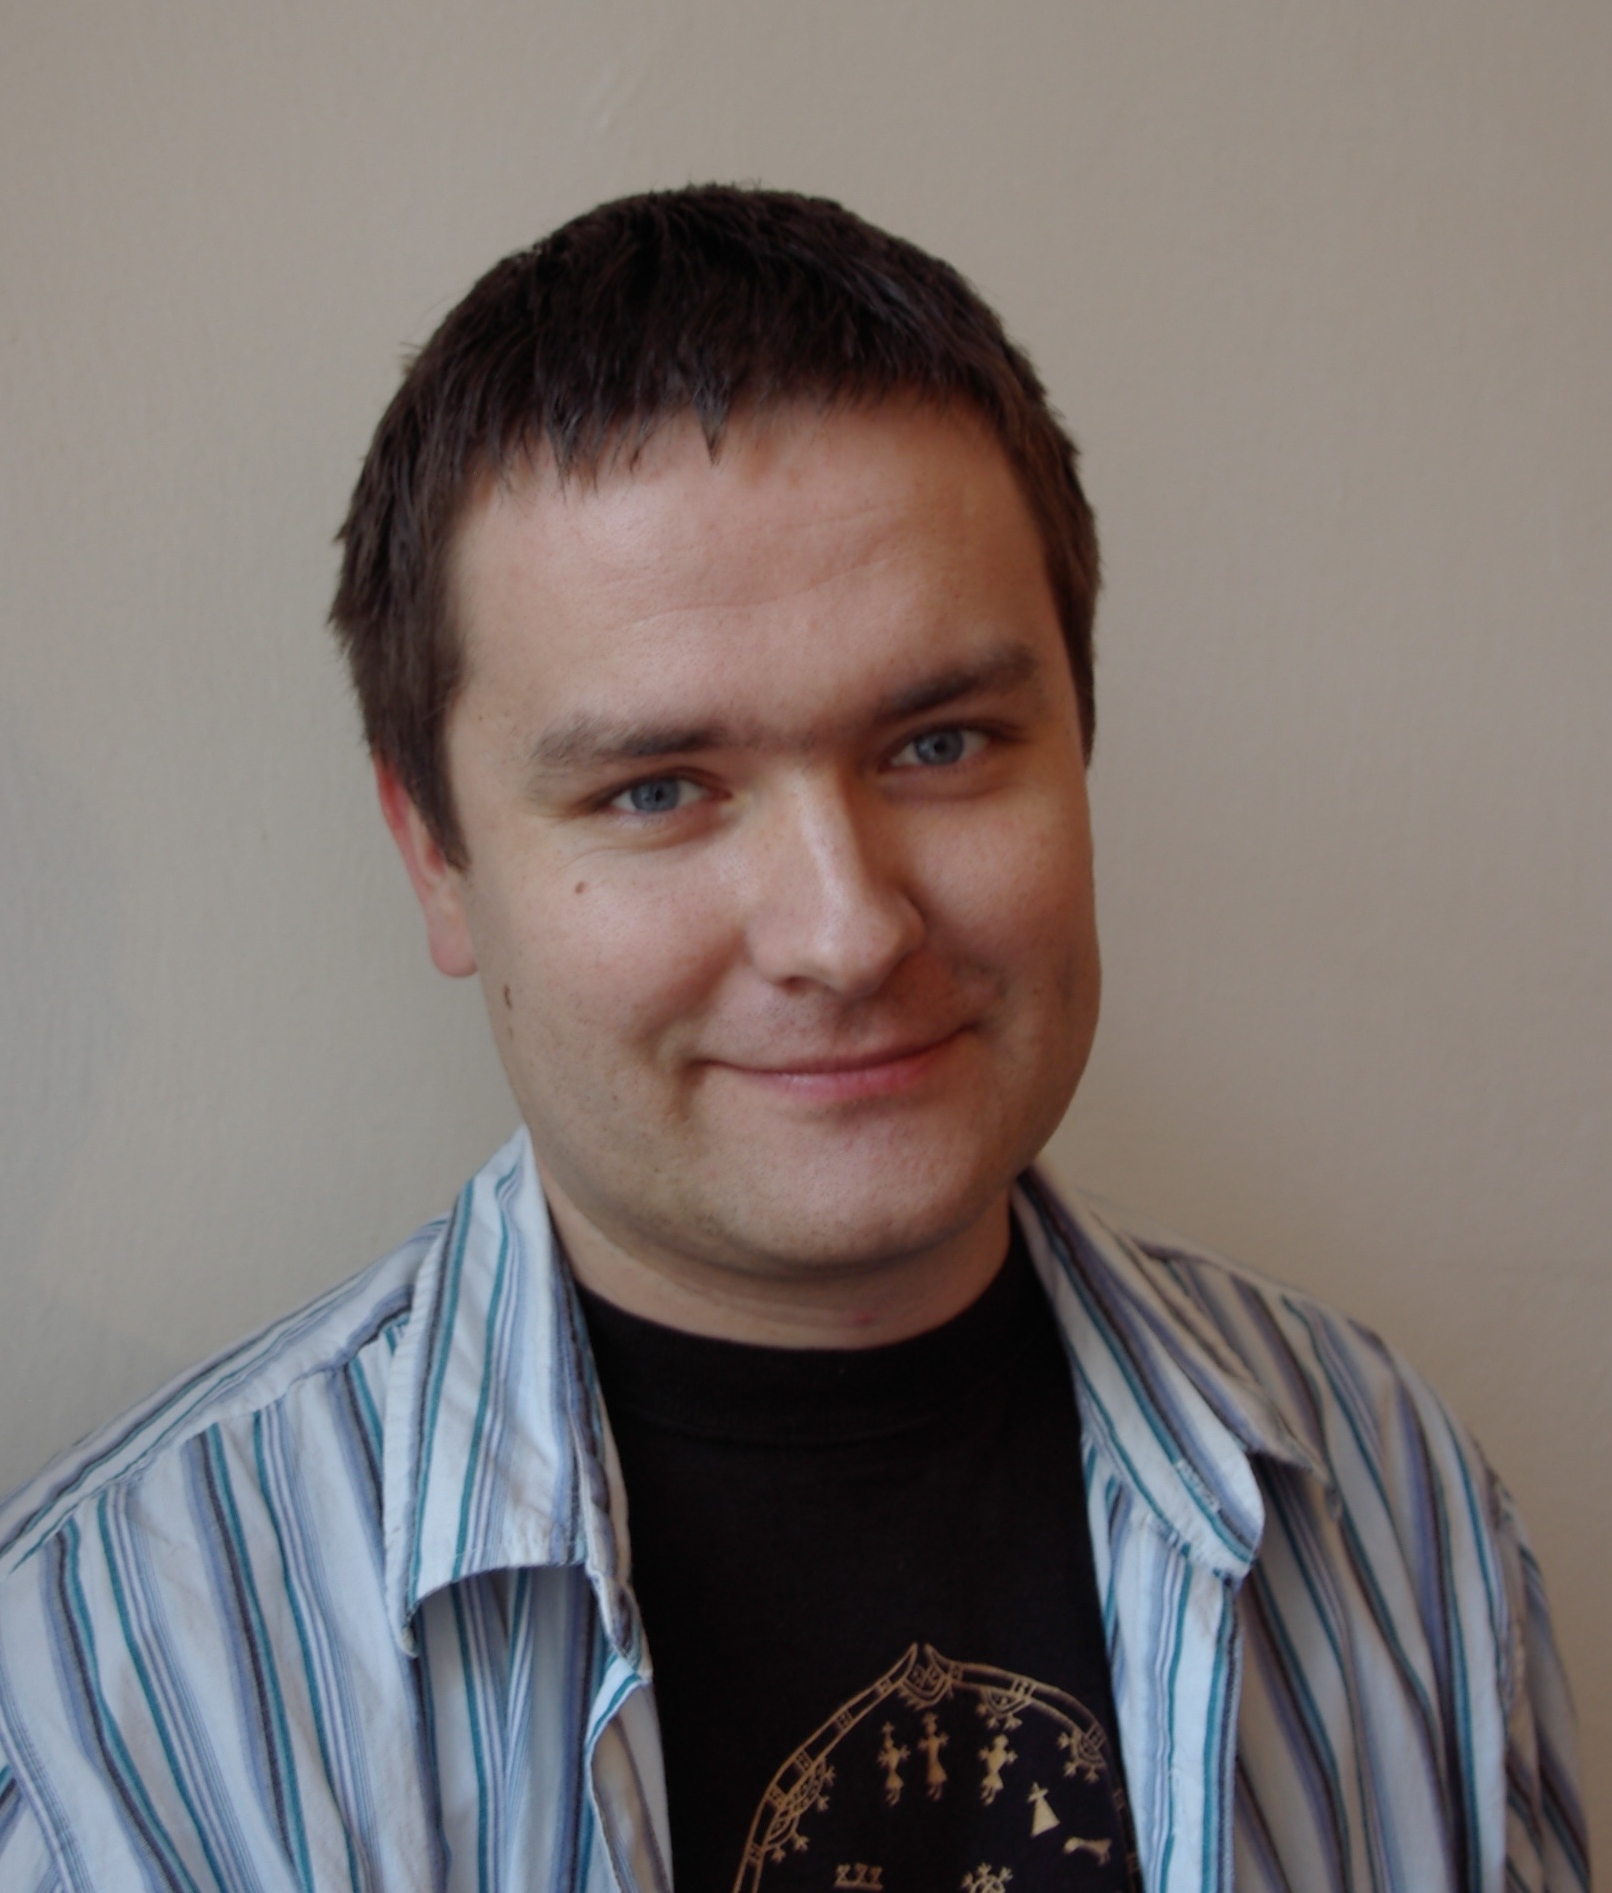
\includegraphics[width=4cm,height=5cm,keepaspectratio]{invited_img/szymczak}
		\end{center}
		\vspace{-20pt}
		\vspace{-10pt}
	\end{wrapfigure}
	Piotr Szymczak received his Ph.D. from the University of Warsaw (Poland) in 2001. After two years of postdoctoral research at the University of Florida he joined the Institute of Theoretical Physics at the University of Warsaw as an assistant professor. His research focuses on the intersection between fluid dynamics and other fields: from the dissolution of porous or fractured rock to the structure and dynamics of biological soft matter. The approach taken is to model the system in a simple but physically meaningful way, and then explore the model using the combination of analytical and numerical techniques.
	
	\section*{Abstract}
	
	The waves of the sea, the little ripples on the shore, the sweeping curve of the sandy bay between the headlands, the outline of the hills, the shape of the clouds, all these are so many riddles of form, so many problems of morphology, and all of them the physicist can more or less easily read and adequately solve" - wrote D'Arcy Wentworth Thompson in 1917 in his famous book "On growth and form". Modern physics has progressed along the way outlined by Thompson, discovering the principles by which multiplicity of relatively simple interactions can give rise to the emergence of organized structures or qualitatively new behaviors. In this talk, I will give two examples of self-organizing growth processes driven by the flow: the growth of "wormholes" in a dissolving rock during early stages of cave formation and the growth of seepage channels incised by groundwater flow. In particular, I will discuss the question why the initially planar fracture is dissolving in an inhomogeneous manner, leading to the appearance of karst conduits and why the tributaries of Apalachicola river in Florida join each other at an angle of 72 degrees.
    \vspace{.5cm}
    \newpage
    
